\chapter{Non Real-time scheduling algorithms}
Lo \textit{scheduling} è l'attività che permette di selezionare quale processo o \textit{thread} bisogna eseguire come successivo. In generale nei sistemi operativi, possiamo distinguere tre tipologie di \textit{scheduling}:
\begin{itemize}
    \item \textbf{\textit{long term scheduling}}: prima di creare il processo, viene deciso se attivarlo o meno. Viene implementato tramite un \textbf{test di ammissione}, se il processo passa questo controllo allora viene inserito nella \textit{ready queue}, se no viene interrotto finché non gli viene permesso di essere \textit{schedulato} [ se il \textit{load} del processore è troppo alto il nuovo task rischia di essere solo di ``intralcio'' ].
    \item \textbf{\textit{medium term scheduling}}: permette di decidere se un processo deve essere \textit{preemptato} o meno.
    \item \textbf{\textit{short term scheduling}}: decide quale processo deve essere eseguito come successivo. Possiamo distinguere:
    \begin{itemize}
        \item \textbf{\textit{selection function}}: decide quale processo viene selezionato dalla \textit{ready queue}, seguendo alcune regole.
        \item \textbf{\textit{decision mode}}: quando la decisione è stata presa si può comportare in maniera \textbf{\textit{preemptive}} oppure \textbf{\textit{non-preemptive}}.
    \end{itemize}
\end{itemize}
\textbf{\textit{Scheduling Criteria}}: come si possono valutare le performance di uno \textit{scheduler}:
\begin{itemize}
    \item \textbf{\textit{user-oriented}}: si va ad analizzare il \textit{response-time} del processo.
    \item \textbf{\textit{system-oriented}}: si va ad analizzare il \textit{throughput}, ovvero quanto lavoro il sistema può eseguire in un certo intervallo di tempo.
\end{itemize}
Per quanto le performance siano importanti in certe circostate ci possono interessare la \textbf{predicibitilà} (\textit{real-time system}) o la \textbf{\textit{fairness}}. \\
Tra i processi possiamo differenziare anche il tipo di risorsa che viene utilizzanta: \textbf{\textit{CPU-Bound}} e \textbf{\textit{I/O Bound}}, nel primo caso il processo è orientato a lavorare sul processore, mentre nel secondo caso i processi possono essere in attesa di un \textit{I/O device}. La stragrande maggioranza dei processi è un mix dei due. \\ \newline
Uno \textit{schedule} $\sigma$ si dice \textbf{fattibile} (\textbf{\textit{feasible}}) se tutti i \textit{tasks} sono capaci di completare entro un insieme di vincoli. \\
Un \textit{tasks set} $\mathcal{T}$ si dice \textbf{\textit{schedulable}} se esiste uno \textit{schedule} fattibile per esso. \\ \newline
\textbf{\textit{The General Scheduling Problem}}: dato un \textit{tasks set} $\mathcal{T}$ di $n$ \textit{tasks}, un set $\mathcal{P}$ di $m$ processori e un set $\mathcal{R}$ di $r$ risorse, trovare un assegnamento di $\mathcal{P}$ e $\mathcal{R}$ per $\mathcal{T}$ che produce uno \textit{schedule} fattibile. \\
È stato dimostrato nel 1975 da Garey e Johnson che il \textit{general scheduling problem} rientra nella categoria \textbf{\textit{NP hard}}. È però possibile, rilassando i vincoli e specificando certe condizioni, ricordurci ad un algoritmo \textit{polynomial time}. \\
Per il ora consideriamo:
\begin{itemize}
    \item processore singolo
    \item \textit{fully preemptive tasks}
    \item attivazione simultanea
    \item nessun vincolo di precedenza
    \item nessun vincolo sulle risorse
\end{itemize}

\begin{tabular}{ |p{7.25cm}|p{7.25cm}| }
    \hline
    \multicolumn{2}{|c|}{\textbf{Algorithm taxonomy}} \\
    \hline
    \textbf{\textit{preemptive}} & \textbf{\textit{non-preemptive}} \\
    \hline
    \textbf{\textit{off line}}: & \textbf{\textit{on line}}: \\
    tutte le decisioni sullo scheduling vengono prese prima dell'attivazione dei task, normalmente lo \textit{schedule} viene salvato in una tabella (\textbf{\textit{table-driven scheduling}}) & le decisioni di scheduling vengono prese \textit{runtime} sul set dei tasks attivi \\ \hline
    \textbf{\textit{static}}: & \textbf{\textit{dynamic}}: \\
    le decisioni di scheduling vengono prese basandosi su parametri fissati, staticamente assegnati al task prima dell'attivazione & le decisioni di scheduling vengono prese su parametri che possono variare nel tempo \\ \hline
    \textbf{\textit{optimal}}: & \textbf{\textit{best effort}}: \\
    trova sempre uno \textit{schedule} fattibile, se \textbf{esiste} & fa del suo meglio per trovare uno \textit{schedule} fattibile, se esiste, ma non lo garantisce. \\ \hline
\end{tabular}
\\ \newline
Le \textit{policies} classiche di \textbf{\textit{scheduling}}, che però non sono adatte per sistemi \textit{real-time}, sono:
\begin{enumerate}

    \item \textbf{\textit{First Come First Served} (FCFS)}: assegna l'utilizzo della CPU al task basandosi sull'ordine di arrivo, non è \textit{preemptive}, è dinamico, online e \textit{best effort}. \\
    $\rightarrow$ molto \textbf{impredicibile}: il \textit{response time} è fortemente dipendente dall'ordine di arrivo dei task.

    \item \textbf{\textit{Shorter Job First} (SJF)}: seleziona il task che ha il minor \textit{computational time}, può essere sia \textit{preemptive} che \textit{non-preemptive}, è statico (il parametro $C_i$ è fissato da configurazione), può essere usato sia \textit{online} che \textit{off-line} e permette di minimizzare la \textit{response time} \textbf{media}. \\
    \textcolor{green}{\textbf{Dimostrazione dell'ottimalità di SJF}}: consideriamo uno scheduler $\sigma \neq \text{SJF}$ e un'altro scheduler $\sigma'$ che è uguale a SJF fino all'istante $f_s$
    \begin{figure}[h]
        \centering
        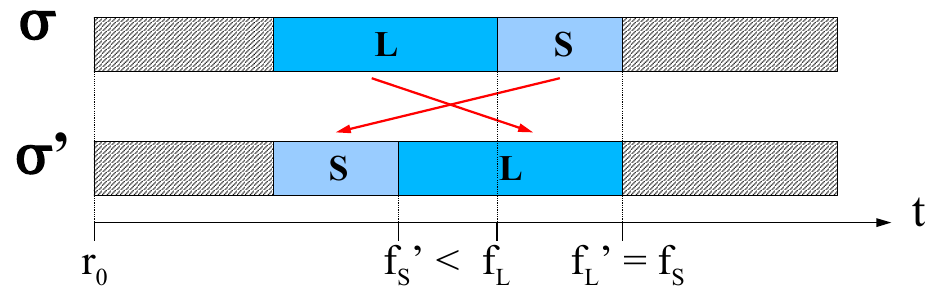
\includegraphics[width=0.4\textwidth]{img/sjf_opt}    
    \end{figure}
    \\ 
    Presi due task $L$ e $S$ che hanno \textit{request time} $r_i \; i \in \{L, S\}$ e \textit{finish time} $f_i \; i \in \{L, S\}$. Lo \textit{schedule} $\sigma$ schedula il task $L$ prima (non conforme con SJF), mentre $\sigma'$ schedula il task $S$ come primo (conforme a SJF). Possiamo dire che $f'_L = f_S$ in quanto la somma del tempo dei due task non cambia, ma cambia solo l'ordine di schedulazione. È intuitivo che il \textit{finish time} del primo task è però sbilanciato verso lo scheduler $\sigma'$ infatti avremo $f'_S < f_L$. \\
    Avremo perciò $f'_S + f'_L \leq f_S + f_L$ 
    \begin{center}
        $\rightarrow \qquad \bar{R}(\sigma') = \frac{1}{n} \cdot \sum_{i = 1}^{n}{(f'_i - r_i)} \leq \frac{1}{n} \cdot \sum_{i = 1}^{n}{(f_i - r_i)} = \bar{R}(\sigma)$
    \end{center}
    Lo scheduler $\sigma'$ è equivalente a SJF solo fino all'istante $f'_L = f_S$, bisogna andare quindi ad iterare su ogni scheduler $\sigma \in \{\sigma', \sigma'', ..., \sigma^*\}$, andando a riproporre l'analisi appena condotta avremo che: $\bar{R}(\sigma) \geq \bar{R}(\sigma') \geq \bar{R}{\sigma''} \geq \cdots \geq \bar{R}(\sigma^*)$ \\
    $\rightarrow$ $\sigma^* = \sigma_{sjf}$ e quindi avremo che $\bar{R}(\sigma_{SJF})$ è la \textbf{minima \textit{response time} media} ottenibile da ogni \textbf{algoritmo}. \\
    \textbf{SJF non è un algoritmo fattibile per il \textit{Real-Time}}.

    \item \textbf{\textit{Priority Scheduling}}: ad ogni task viene assegnata una \textbf{priorità}, il task con la priorità maggiore viene eseguito come primo, mentre per i task con pari priorità siene eseguito uno scheduler o FCFS o RR. Può essere utilizzato per fini \textit{real-time} se le priorità sono assegnate seguendo specifiche regole. Lo \textit{scheduler POSIX} è uno scheduler con 99 priorità. Può essere sia statico che dinamico.
    \begin{itemize}
        \item può avere problemi di \textbf{\textit{starvation}} infatti dei task a bassa priorità possono accumulare ritardo per via della \textit{preemption} dovuto a task con più alta priorità.
        \item Una possibile \textbf{soluzione} è quella dell'\textbf{\textit{aging}} ovvero che la priorità viene incrementata con il passare del tempo: \\
        \begin{center}
            $p_i \propto \frac{1}{C_i} \simeq \text{SJF}$ \\ 
            $p_i \propto \frac{1}{r_i} \simeq \text{FCFS}$
        \end{center}
    \end{itemize} 

    \item \textbf{\textit{Round Robin}}: la \textit{ready queue} viene servita con un \textbf{FCFS}, ma il sistema conosce il concetto di \textbf{\textit{time quantum} (Q)}, ogni task $\tau_i$ non può eseguire più un \textbf{Q} unità di tempo. Quando \textbf{Q} scade, $\tau_i$ viene riaccodato nella \textit{ready queue}.
    \begin{figure}[h]
        \centering
        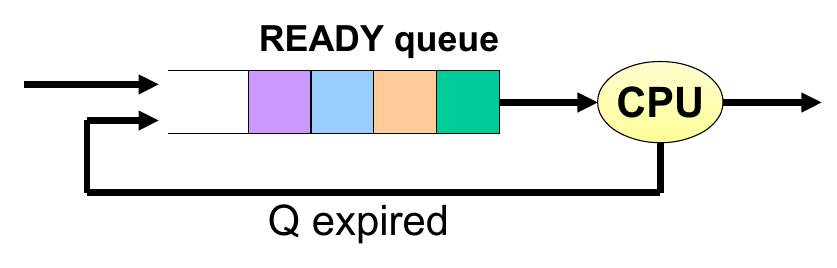
\includegraphics[width=0.4\textwidth]{img/rr}
    \end{figure}
    \\
    Introduce il concetto di \textbf{\textit{time sharing}}: ovvero che ogni task esegue in solitaria su un ``processore virtuale'' $n$ volte più lento rispetto a quello reale.
    \begin{center}
        $R_i \simeq (n\mathcal{Q}) \frac{C_i}{\mathcal{Q}} = nC_i$
    \end{center}
    Se $Q > \max(C_i)$ allora RR $\equiv$ FCFS, e se consideriamo che ogni volta che viene \textit{preemptato} un task bisogna eseguire un \textit{context switch} definito da un tempo $\delta$ allora avremo che:
    \begin{center}
        $R_i \simeq n \cdot (\mathcal{Q} + \delta) \frac{C_i}{\mathcal{Q}} = nC_i \cdot (\frac{\mathcal{Q} + \delta}{\mathcal{Q}})$
    \end{center}

    \item \textbf{\textit{Multiple-feedback Queues}}: questo \textit{scheduler} consiste in: $N$ code, ognuna delle quali viene ordinata tramite FIFO a unità di tempo \textit{quantum} fisse. Lo \textit{scheduler} sceglie il primo processo dalla coda con più alta priorità e imposta un timer a \textbf{Q}. Consideriamo $\text{RQ}_k$ come la coda priorità maggiore che ha un task pronto per essere eseguito. Se il processo viene completato entro o si blocca prima che il scada bisogna selezionare il processo successivo dalla coda con più alta priorità e impostare il timer, se no sposta il processo nella coda $\text{RQ}_{k + 1}$. Quindi in maniera periodica, se un processo non viene completato allora viene ``spostato'' nella priorità più alta (questo viene fatto per evitare \textit{starvation}).
    \begin{figure}[h]
        \centering
        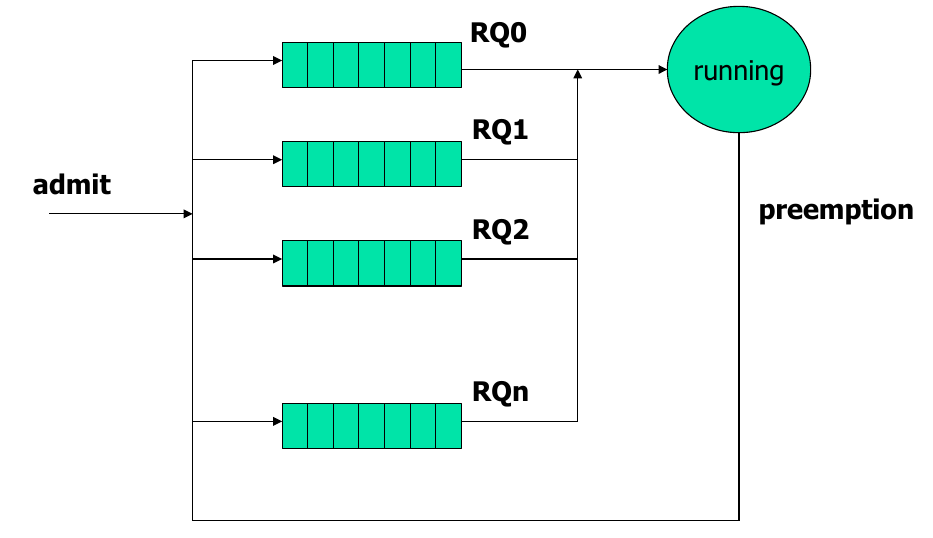
\includegraphics[width=0.5\textwidth]{img/mfq}
    \end{figure}
\end{enumerate}